\chapter{Sample Generation}
\label{sec:sampling}

Our objective is to conduct a systematic investigation of sample generation methods, driven by the desire to comprehend the impact of each modification on the performance of the sampling strategies. We explore the effects of each component in sample generation and propose new strategies to improve the performance of the learned heuristic. By systematically analyzing and comparing the outcomes of each strategy, we can gain valuable insights into the strengths and weaknesses of different sample generation approaches. This understanding will enable us to identify the key factors that contribute to improved performance and guide us to a better learned heuristic function.

Therefore, we focus on how three aspects of sample generation influence the performance of the learned heuristic to guide a search algorithm: the distribution of states $s_i$ in the state space part of the sample set, the quality of the estimates $h_i$ of samples with respect to the $\hstar$-value, and the methods that generate sample sets. In our setting, learning a heuristic function requires a set of samples $(s_1,h_1),\ldots,(s_N,h_N)$, where each sample $(s_i,h_i), i\in[N]$ consists of a state $s_i$ and a cost-to-goal estimate $h_i$.

We restrict our study to generalizing over planning tasks with initial states part of the same forward state space and a fixed goal condition. We study model-free approaches with access to predecessors and successors of partial states through a black-box function, the goal condition, and the domain of each variable. We also study model-based approaches that have access to mutexes derived from a \sas model. We approach first, in Section~\ref{sec:generation}, the generation of states, and then, in Section~\ref{sec:hvalue}, the estimation of the cost-to-goal. In both sections, we discuss approaches from the literature and introduce new methods. The new methods are a novel sampling strategy combining regression by breadth-first search with random walk, an adaptive regression limit, and two improvement methods for cost-to-goal estimates. Finally, we present the complete workflow of our algorithm and an example.

\section{Generation of States}
\label{sec:generation}

Unlike other domains in machine learning, such as image recognition or natural language processing, where datasets of samples are often collected in real-world experiments and subsequently need to be manually annotated and carefully curated, the task of sample generation in the field of classical planning presents a distinct challenge. In contrast to the reliance on external data sources, classical planning leverages the structure and characteristics of the task domain itself. In this context, the generation of samples becomes an algorithmic problem that capitalizes on the availability of the state space and the ability to compute cost-to-goal estimates. This capability allows exploring various techniques using only computational resources.

The algorithmic nature of sample generation in classical planning not only provides a systematic and controlled approach but also enables the exploration of diverse sample distributions. Approaches from the literature to generate states generally revolve around three key approaches: progression from one or more initial states, random sampling of the state space, or regression from the goal state.

Both progression and regression involve starting from a state and systematically applying forward (progression) or backward (regression) operators to explore the state space. This iterative process gradually expands the set of generated states, effectively capturing the dynamics and potential paths within the task. Various expansion strategies can be employed, such as random walks, breadth- or depth-first searches, or teacher searches which include ``on policy'' searches in methods using reinforcement learning or bootstrapping~\cite{Arfaee.etal/2011}. These strategies influence the coverage and exploration patterns of the generated states, impacting the overall diversity and representation of the sample set.

A problem in both progression-based methods and random sampling is obtaining the cost-to-goal estimates. Without access to efficiently computable heuristic functions, or in model-free approaches, obtaining these values is a challenging task. Typically, search algorithms need to be employed to generate these estimates, which can introduce significant computational costs, especially in tasks with large sizes.

To remain less dependent on models than logic-based methods and also more general, we focus on regression for which an upper bound on the cost-to-goal is readily available, discussed in Sections~\ref{sec:sampling-generation}~and~\ref{sec:rollout-depth-limit}. Still, regression leads to partial states, so the problem of generating complete states is addressed in Section~\ref{sec:sample-completion}. Use random sampling as an additional approach is also discussed in Section~\ref{sec:random-samples-theory}.

\subsection{Sampling by Regression}
\label{sec:sampling-generation}

To generate samples, we expand the backward state space through regression. We address the main techniques in the literature such as expansion by BFS, DFS and random walk. The sampling process is carried out by performing regression rollouts, which consist of a series of state expansions. The rollout continues until the last expanded state has no predecessors or, particularly for random walk, the depth limit $L$ is reached. Therefore, random walks can have multiple rollouts, while \bfs and \dfs only have one -- except if the number of states in the backward state space is less than $N$, in which case they need to perform more than one rollout to ensure the number of samples for training. The sampling generation process stops when the number of required samples $N$ has been reached.

During expansion, we optionally use mutexes obtained from an analysis of the planning task -- in our case as computed by Fast Downward~\cite{Helmert/2006} -- to discard partial states which cannot be completed to complete states without violating a mutex, as described in Section~\ref{sec:sample-completion}. We also discard repeated partial states for random walk rollouts, such that a single rollout never cycles. However, it is possible for the same partial state to be sampled multiple times in different rollouts.

Regression starts from the goal state $s^*$ with the cost-to-goal estimate~$h(s^*)=0$. When applying a backward operator $o$ to a state~$s$, the resulting state~$s' = \pred(s, o)$ receives a cost-to-goal estimate of $h(s') = h(s) + \text{cost}(o)$. For a state $s$ generated during rollout that satisfy the goal condition, i.e., $s \subseteq s^*$, we set its cost-to-goal estimate to $h(s) = 0$. States are added to the sample set when generated in the random walks and when expanded in BFS and DFS. In all methods, operators backward applicable to a state are applied in random order.

By utilizing different expansion strategies and considering multiple rollouts, we aim to generate a diverse and representative sample set of the state space. Different expansion strategies generate sample sets with varying frequencies of optimal distances from the goal. In our experience, good coverage of states close to the goal, such as those obtained by BFS or random walks, is useful, as is the greater depth obtained by DFS or random walks. However, random walks from the goal often sample states close to the goal multiple times, and DFS can lead to a concentration of distant samples from the goal. Based on these observations, we propose a novel combination of BFS and random walks called \bfsrw that aims to have a good coverage close to the goal and a diverse set of samples from the remaining state space.

We propose the \bfsrw algorithm, which combines the strengths of breadth-first search and random walks to generate a diverse and representative sample set. \bfsrw addresses the limitations of individual strategies by leveraging BFS for good coverage of states close to the goal and random walks for exploring distant regions. By strategically integrating these approaches, \bfsrw aims to achieve a balanced and comprehensive sampling of the state space. Algorithm \ref{alg:fsm} presents the approach.

\begin{algorithm}[h]
    \SetAlgoLined

    \SetKwData{Empty}{\{\}}
    \SetKwData{N}{N}
    \SetKwData{Nbfs}{N\textsubscript{bfs}}
    \SetKwData{bfspct}{p\textsubscript{\bfsrw}}
    \SetKwData{initstate}{s\textsubscript{0}}
    \SetKwData{S}{S}
    \SetKwData{Di}{D\textsubscript{k}}
    \SetKwData{Dj}{D\textsubscript{k+1}}
    \SetKwData{s}{s}
    \SetKwData{sp}{s'}
    \SetKwData{t}{t}
    \SetKwData{O}{Q}
    \SetKwData{L}{L}
    \SetKwData{Srw}{S\textsubscript{RW}}

    \KwData{
        \N: number of samples;
        \bfspct: fraction of samples obtained by BFS;
        \initstate: initial state;
        \L: random walk rollout limit
    }
    \KwResult{\S: the sample set}
    \SetKwProg{Fn}{Function}{:}{}

    \SetKwFunction{FSM}{FSM}
    \Fn{\FSM{\bfspct, \initstate, \L}}{
        $\S \gets \{\initstate\}$ \\
        $\O \gets \{\initstate\}$ \\
        $\Di \gets \{\initstate\}$ \\
        $\Dj \gets \Empty$ \\
        $\Nbfs \gets \N \times \bfspct$ \\

        \tcp{BFS phase}
        \While{$\lvert \S \rvert < \Nbfs$ \textnormal{\textbf{and}} $\Di \neq \emptyset$}{
            Shuffles \Di \\
            \ForEach{$\s \in \Di$}{
                $\t \gets \{\sp \mid \sp \in pred(s)\ \textbf{and}\ \sp \notin \S$\} \\
                \If{$\lvert \S \rvert + \lvert \t \rvert \le \Nbfs$}{
                    $\Dj \gets \Dj \cup \t$ \\
                    $\S \gets \S \cup \t$ \\
                    $\O \gets \left(\ \O \cup \t\ \right) \backslash\ \{\s\}$ \\
                }
            }
            $\Di \gets \Dj$ \\
        }

        \tcp{RW phase}
        \While{$\lvert \S \rvert < \N$}{
            Shuffles \O \\
            \ForEach{$\s \in \O$}{
                $\Srw \gets$ set of $min(\L - h(\s), \N - \lvert \S \rvert)$ states sampled via RW starting from $\s$ \\
                $\S \gets \S \cup \Srw$ \\
                \lIf{$\lvert \S \rvert = \N$}{break}
            }
        }

        \Return \S \\
    }

    \caption{FSM algorithm}
    \label{alg:fsm}
\end{algorithm}

\bfs has two phases. In the first phase, a fixed percentage~$p_\bfsrw$ of the desired $N$ samples is generated using BFS. (Note that $p_\bfsrw$ can additionally represent time and memory limitations -- in this case, \bfs stops once either of them is reached first.) The \bfs expands a state from layer~$k$ that generates $n$ states from layer~$k+1$ (line 10). These generated states are sampled only if the current total samples plus $n$ are within $p_{\bfsrw}N$ samples; otherwise, no states are sampled and \bfs expands another state. When expanding an entire layer, the algorithm moves to the next layer.

Let $Q$ be the states of the set of samples that have not been expanded. The second phase generates multiple random walk rollouts, each starting from a state in $Q$ chosen randomly with a complete replacement only after all states have been selected once. This is repeated until reaching $N$ samples in the sample set. During a random walk, states sampled in the BFS phase are discarded. This approach is compared to traditional ones in Subsection~\ref{sec:experiment1-subset}.

\subsection{Maximum Regression Limit}
\label{sec:rollout-depth-limit}

The maximum regression limit plays a crucial role in controlling the depth of state exploration during the sampling process. In essence, this limit determinates how far the sampling can deviate from the goal state during regression. For example, in random walk represents the maxium number of random steps that the algorithm takes in a walk (rollout). In BFS or DFS, the maximum regression limit corresponds to the maximum depth level that can be reached.

This limit serves two main objectives. First, particularly in regression-based methods, it helps maintain the precision of the cost-to-goal estimate, which is determined by the distance from the goal state that the sample was generated and tends to degrade during sampling due to the random nature of algorithms such as random walk or DFS. Secondly, it regulates the distribution of samples by periodically restarting the sampling process, effectively distributing them across the different distances from the goal state.

By establishing an appropriate maximum regression limit, we can achieve a balance between exploration and precision in the sampling process. If the limit is set too low, the sampling may fail to cover areas that are far from the goal state, typically where the initial states of a search reside, resulting in a sample set lacking information from these regions. On the other hand, if the limit is excessively large, the sampling may extend too far from the goal state, thereby compromising the accuracy of the cost-to-goal estimate.

A simple strategy is to define some maximum limit, deonoted as $L$. This has been used in previous work, e.g.,~by Yu et al.~(\citeyear{Yu.etal/2020}) and O'Toole et al.~(\citeyear{OToole/2022}) with $L=200$ and $L=500$, respectively. A fixed limit is not the optimal choice for tasks with state spaces of different diameters or different maximum distances to a fixed goal when we aim for a representative sample of the state space.

To address this challenge, it is necessary to use adaptive strategies that dynamically adjust the maximum expansion depth based on the characteristics of the state space. This adaptability ensures that the sampling process can accommodate variations in the diameter of the state space and the maximum distance to a goal, facilitating the generation of a representative sample set that encompasses regions of the entire state space.

The most effective maximum regression limit for a fixed goal should be defined as a function of the longest distance \distfarthest from the goal state to any other potential initial state. For BFS, \distfarthest would be the ideal estimate; for DFS and random walks, higher limits are required since they do not follow the shortest paths.
Since \distfarthest, in general, is unknown, a potential solution is to estimate this value using available or domain-specific information.

We propose two adaptive and approximated methods to define a suitable maximum regression limit based on the input task parameters. The first method, model-free, is the number of facts in the task $F=|\mathcal{F}(s_0)|$. This approach provides an estimate that takes into account the assumption that if at least one fact is changed at each step, the worst-case scenario, requiring a change in all facts, would take $F$ steps.

The second method, on the other hand, is model-based and defined as the number of facts per mean number of effects in the operators, i.e., $\bar F=\ceil{\facts/\overline{\eff}}$ where $\overline{\eff}=\sum_{o\in \mathcal{O}} |\eff(o)|/|\mathcal{O}|$. This technique generates an approximate estimate of the diameter of the state space considering that, in the worst case, we need to set all propositions of a state to reach the goal state, and we can set on average $\overline{\eff}$ propositions per given step, so we need to take $\bar F$ steps to traverse the state space.

By employing these adaptive and approximated methods, we can define the maximum regression limit based on the characteristics of each planning task. The model-free method offers a simple yet effective estimation, while the model-based one provides a more nuanced approximation. These approaches allow for the adaptability of the maximum regression limit, enabling a more tailored and accurate sampling process.

\subsection{Sample Completion}
\label{sec:sample-completion}

The goal state is represented as a partial state, consisting of a subset of facts of a complete state that needs to be satisfied to reach the desired solution. Therefore, sampling by regression generates a set of partial states. Since NNs rely on complete states as input during the search, it becomes necessary to perform state completion, which involves assigning values to the missing facts in the partial states.

We present three approaches to complete a partial state. The first one involves random assignment, where each partial state can be completed by assigning a value $s(v)\in\dom(v)$ to all fact pairs $(v,s(v))$ where $s(v)=\bot$. This completion strategy, which relies solely on the available domain values without making any additional assumptions, can be considered a model-free approach.

The second method are model-based and utilizes mutexes to generate complete states that are more similar to those encountered during the search. This method also assigns a random value $s(v)\in\dom(v)$ to each undefined variable $v$ but excludes states that do not satisfy mutexes derived from the planning task. This is achieved by rejection sampling, where the undefined variables are processed in random order and set to a random value that does not violate the mutexes. If the state could not be completed in $10$\,K trial orders, we leave the facts undefined, i.e., set to false\footnote{Empirically this case is negligible since it occurs in about $0.1\,\%$ of the samples, in four of nine domains.}. By incorporating the mutex information, we generate more comprehensive and coherent complete states, enhancing the accuracy and quality of the training data provided to the NN.

While this model-based solution utilizing mutexes offers improved state completion, it is still possible for generate invalid states or states that cannot be reached during the search. To investigate the impact of generating only those states that are reachable from the initial states of interest, we introduce an ideal state completion method. This method aims to produce a sample set that are highly relevant to the specific task. To complete a partial state $s$ we sample a random state from $s~\cap$~\fssp. Since we sample by regression, for some states, $s~\cap$~\fssp may be empty; such states are discarded during regression. However, it is important to note that this method is applicable only to small tasks where we can enumerate the complete forward state space \fssp of the initial state~$s_0$.

By leveraging additional information and making more informed decisions during the state completion, we can investigate the gain that a more informed approach can have on the learning and reasoning of the NN.

\subsection{Randomly Generated Samples}
\label{sec:random-samples-theory}

We explore the random sampling, as proposed by O'Toole et al.~(\citeyear{OToole/2022}), as an additional approach to generate samples. They have shown that adding randomly generated samples to a set of samples generated by expansion improves the performance of the search algorithm guided by the learned heuristic. In their work, they propose to set the cost-to-goal estimate for randomly generated samples to $L+1$ for a maximum regression limit of $L$.

We adopt this method to investigate the impact of randomly generated samples on the sampling process. These samples are generated from fully undefined states using the model-based technique described in the previous section. When generating a state~$s$ by random sampling, if $s$ is already present in the sample set, i.e.,~$s = s_i$ for some $i\in[N]$, it receives the same cost-to-goal estimate $h_i$, otherwise it receives a cost estimate of $1+\max_{i\in[N]} h_i$ that is larger than all sample estimates.

By incorporating random sampling into our study, we aim to investigate their influence on the overall performance of the sampling approach. The introduction of randomly generated samples contributes to diversifying the sample set, encompassing a wider range of states within the state space. This diversity can potentially enhance the robustness and generalization capabilities of the learned heuristic, enabling more effective and efficient outcomes. For simplicity, from this point on we refer to randomly generated samples as ``random samples''.

\section{Improving Cost-to-Goal Estimates}
\label{sec:hvalue}

The quality of the sample set is also influenced by the accuracy of the cost-to-goal estimate. Accurate cost-to-goal estimates ($h$-values) help to improve the performance of the learned heuristics, and thus reduce the number of expanded states during a search. Note that while it is generally expected that better $h$-value estimates result in more reliable heuristic functions, leading to more efficient search, this relationship is not always guaranteed \cite{Holte/2010}.

To improve the cost-to-goal estimate, our objetive is to approximate the true cost-to-goal estimate \hstar. Our sampling approach ensures that the cost-to-goal estimates assigned to the samples are based on the operators used to reach that particular state. Thus, we guarantee that a sample never underestimate the \hstar.

\begin{property}
    \label{prop:hvalue}
    The cost-to-goal estimate $h(s)$ of a sample $s$ obtained by regression satisfies $h(s)\geq h^*(s)$.
\end{property}
\begin{proof}
    This follows simply because each estimate is witnessed by a plan. As observed in Chapter~\ref{sec:preliminaries}, a valid regression sequence $\rho=(o_1,\ldots,o_k)$ generates a sequence of partial states that can reach the goal in at most $k$ steps and with cost at most $\sum_{i\in[k]}\text{cost}(o_i)$, which cannot be lower than the optimal cost.
\end{proof}

Therefore, we apply two simple procedures that improve the cost-to-goal estimates but maintain \cref{prop:hvalue}. The first, dubbed \hmin, minimizes estimates over repeated samples, and the second, \hvfc, over successors of samples.

\subsection{Improvement of Repeated Samples}
\label{sec:hmin} 

When generating samples through multiple rollouts, there is a possibility of overlap, where the same state could appears at different distances across different rollouts, leading to varying cost-to-goal estimates. This introduces a challenge when training the NN as different labels for the same sample can result in inconsistency and affect the learning process. To address this issue and improve the quality of cost-to-goal estimates, we employ a technique called Sample Improvement (SAI).

SAI aims to improve the consistency and reliability of the training data by selecting a single cost-to-goal estimate for each unique state. \cref{prop:hvalue} guarantees that no sampled cost-to-goal estimate underestimates \hstar, so the smaller its value the closer it is to the true cost-to-goal. Therefore, we choose the sample with the lowest cost-to-goal estimate as the representative for each particular state, as follows.

For all sampled states $s$ we update each cost-to-goal estimate to the best estimate $h(s) = \min\{h_i \mid s=s_i, i\in[N]\}$. Since different partial states can generate identical complete states, the improvement is applied to partial states as well as complete states. Choosing the minimum $h$-value is clearly sound since, in all cases, we have valid plans from a regression that witness these distances; for the same reason, \cref{prop:hvalue} still holds.

\begin{figure}[h]
    \caption[SAI technique applied on a sample set with random walk rollouts.]{SAI technique applied on a sample set with two random walk rollouts. Each node represents a state and each arc an applicable operator. Each rollout has a color and the operators used in it are colored accordingly.}
    \label{fig:sai}
    \addvspace{\baselineskip}
    \centering
    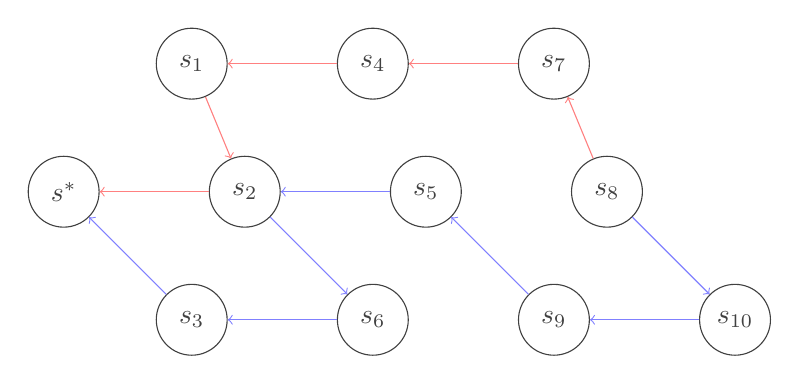
\begin{tikzpicture}[every node/.style={circle, draw}, node distance=23mm, minimum size=9mm]
        \node[color=black!75] (goal) {$s^*$};
        \node[above right of=goal, color=black!75] (s1) {$s_1$};
        \node[right of=goal, color=black!75] (s2) {$s_2$};
        \node[below right of=goal, color=black!75] (s3) {$s_3$};
        \node[right of=s1, color=black!75] (s4) {$s_4$};
        \node[right of=s2, color=black!75] (s5) {$s_5$};
        \node[right of=s3, color=black!75] (s6) {$s_6$};
        \node[right of=s4, color=black!75] (s7) {$s_7$};
        \node[right of=s5, color=black!75] (s8) {$s_8$};
        \node[right of=s6, color=black!75] (s9) {$s_9$};
        \node[right of=s9, color=black!75] (s10) {$s_{10}$};

        \draw[->, color=red!50] (s1) -- (s2);
        \draw[->, color=red!50] (s2) -- (goal);
        \draw[->, color=blue!50] (s2) -- (s6);
        \draw[->, color=blue!50] (s3) -- (goal);
        \draw[->, color=red!50] (s4) -- (s1);
        \draw[->, color=blue!50] (s5) -- (s2);
        \draw[->, color=blue!50] (s6) -- (s3);
        \draw[->, color=red!50] (s7) -- (s4);
        \draw[->, color=red!50] (s8) -- (s7);
        \draw[->, color=blue!50] (s8) -- (s10);
        \draw[->, color=blue!50] (s9) -- (s5);
        \draw[->, color=blue!50] (s10) -- (s9);
      \end{tikzpicture}
\end{figure}

Figure~\ref{fig:sai} presents the technique applied to sampling by random walks. Both rollouts generate the state $s_2$, but through different paths. While the red rollout reaches with a distance of $1$ from the goal state $s^*$, the blue rollout generates $s_2$ after $3$ hops. Consequently, samples have $h(s_2)=1$ and $h(s_2)=3$. By applying the SAI technique, we update the cost-to-goal estimate $h(s_2)$ of both samples to $min(1,3)=1$. The same process is applied to samples of state $s8$, which receives $h(s_8)=min(5,7)=5$.

\subsection{Improvement over Successors}
\label{sec:hvfc}

In addition to sampling the same states in different rollouts, it is also common to sample states that are neighbors in the state space. This is more frequent in states at the beginning of the rollout. By sampling neighboring states, we can leverage the local information to enhance the accuracy of the cost-to-goal estimates. We propose a technique called Successor Improvement (\hvfc).

\hvfc takes advantage of the fact that neighboring samples, with one distance operator, can be connected by this operator to form a new path to the goal, and consequently, a new cost-to-goal estimate. If it produces a shorter path than the current one, we can update to the corresponding cost-to-goal estimate to approximate \hstar. Note that although it is possible to expand the technique to neighbors of two or more distance operators, the computational cost grows exponentially.

\begin{algorithm}[h]
    \SetAlgoLined

    \SetKwData{Empty}{\{\}}
    \SetKwData{S}{S}
    \SetKwData{s}{s}
    \SetKwData{sp}{s'}
    \SetKwData{su}{s'}
    \SetKwData{t}{t}
    \SetKwData{Ms}{A}
    \SetKwData{Mh}{V}

    \KwData{
        \S: the sample set
    }
    \KwResult{\S: the updated sample set}
    \SetKwProg{Fn}{Function}{:}{}

    \SetKwFunction{SUI}{SUI}
    \Fn{\SUI{\S}}{
        Let $\Mh$ be a mapping from state to integer \\
        Let $\Ms$ be a mapping from state to list of states \\
        \ForEach{$\s \in \S$}{
            \If{$\s \notin \Ms$}{
                \lForEach{$\sp \in succ(\s)$}{
                    $\Ms[\s] \gets \Ms[\s] \cup \{\ \t \mid \t \in \S\ \textnormal{\textbf{and}}\ \sp \subseteq \t\ \}$
                }
            }
            $\Mh[\s] \gets min(\Mh[\s], h(\s))$ \\
        }

        \Repeat{no $h$-value to update}{
            \ForEach{$\s \in \Ms$}{
                \ForEach{$\t \in \Ms[\s]$}{
                    \If{$\Mh[\s] > \Mh[\t] + 1$}{
                        $\Mh[\s] \gets \Mh[\t] + 1$ \\
                        $h(\s) \gets \Mh[\s]$
                    }
                }
            }
        }

        \Return \S \\
    }

    \caption{SUI algorithm}
    \label{alg:sui}
\end{algorithm}

The method is detailed in Algorithm~\ref{alg:sui}. Consider directed and labeled graph $G=(V,A)$ where each vertex $s \in V$ corresponds to a sampled partial state and labeled by its lowest cost-to-goal estimate (line 8). For every pair of states $s,t\in V$ such that for some operator $o\in\mathcal{O}$ applicable to $s$ we have $\sucs(s,o)\subseteq t$, we add an arc $(s,t)$ of length $\text{cost}(o)$ to $A$ (line 6). For simplicity, the algorithm is representing a unit cost domain and therefore is not storing the cost of the operators, but they can be stored in line 6 and used in lines 13-14. Also, unlike in regression, if $\pre(o)$ mentions an undefined variable in $s$ then $o$ is not applicable as it generates inconsistencies in forward operators. 

By applying operators on partial states to identify neighboring states from different rollouts, we generate another partial state. A partial state represents a set of complete states. Thus, to determine if a partial state has been sampled, we have to check all its subsets of facts. We maintain a trie data structure, where each sampled partial state is inserted with its facts as a key. When generating a successor $s'$ from $s$ (line 6), we search the trie for sampled partial states $t$ that are supersets of $s'$. Thus, $s$ generates $t$ from the application of an operator and the assignment of zero or more undefined variables, so there is an arc between them.

The second loop (line 10) propagates the value of the cost-to-goal estimate through all possible paths, updating the value of the neighbors (which in the next iteration can update the estimate of their own neighbors and so on). For partial states generated by regression, by construction, at least one successor exists, except for the goal state $s^*$. Therefore, in the worst case, the algorithm will make $L$ iterations, propagating the cost-to-goal estimate of the goal state to the most distant node, working similarly to Dijkstra's Algorithm. As for \hmin, all distances are witnessed by plans, so \cref{prop:hvalue} is maintained.

\begin{figure}[h]
    \caption[SUI technique applied on a sample set with random walk rollouts.]{SUI technique applied on a sample set with two random walk rollouts. Each node represents a state and each arc an applicable operator. Each rollout has a color and the operators used in it are colored accordingly.}
    \label{fig:sui}
    \addvspace{\baselineskip}
    \centering
    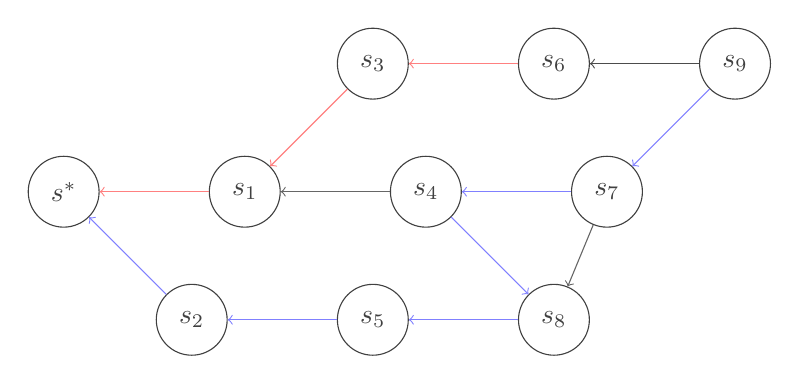
\begin{tikzpicture}[every node/.style={circle, draw}, node distance=23mm, minimum size=9mm]
        \node[color=black!75] (goal) {$s^*$};
        \node[right of=goal, color=black!75] (s1) {$s_1$};
        \node[below right of=goal, color=black!75] (s2) {$s_2$};
        \node[above right of=s1, color=black!75] (s3) {$s_3$};
        \node[right of=s1, color=black!75] (s4) {$s_4$};
        \node[right of=s2, color=black!75] (s5) {$s_5$};
        \node[right of=s3, color=black!75] (s6) {$s_6$};
        \node[right of=s4, color=black!75] (s7) {$s_7$};
        \node[right of=s5, color=black!75] (s8) {$s_8$};
        \node[right of=s6, color=black!75] (s9) {$s_9$};

        \draw[->, color=red!50] (s1) -- (goal);
        \draw[->, color=blue!50] (s2) -- (goal);
        \draw[->, color=red!50] (s3) -- (s1);
        \draw[->, color=black!60] (s4) -- (s1);
        \draw[->, color=blue!50] (s4) -- (s8);
        \draw[->, color=blue!50] (s5) -- (s2);
        \draw[->, color=red!50] (s6) -- (s3);
        \draw[->, color=blue!50] (s7) -- (s4);
        \draw[->, color=black!60] (s7) -- (s8);
        \draw[->, color=blue!50] (s8) -- (s5);
        \draw[->, color=black!70] (s9) -- (s6);
        \draw[->, color=blue!50] (s9) -- (s7);
      \end{tikzpicture}
\end{figure}

Figure~\ref{fig:sui} shows an example of the technique. The rollouts do not overlap but intersect at a distance of one operator between states $s_1$ and $s_4$. This information is discovered by inserting the black arcs to the graph~$G$, which were not previously used by the sampling. From there, we can connect these states to generate a new path from $s_4$ to goal that is shorter than its current one, updating its cost-to-goal estimate from $4$ to $h(s_1)+1=1+1=2$, according to the new path. Now, $s_4$ can update the estimate of its neighbors in the next iteration. Thus, all states generated in the rollout after $s_4$ will be updated. Therefore, although the neighborhood between states is more common close to the goal state, distant states benefit from the propagation of update.

\section{Workflow}
\label{sec:workflow}

Our approach follows the workflow shown in Figure~\ref{fig:workflow}.

\begin{figure}[h]
    \caption{Sample generation workflow.}
    \label{fig:workflow}
    \addvspace{\baselineskip}
    \centering
    \begin{tikzpicture}
        % % side by side
        % \node[draw=black, fill=none, rounded corners, inner sep=5pt] (A) at (0.3,1.3) {Sampling stage};
        % \node[draw=black, fill=none, rounded corners, inner sep=5pt] (B) at (5.3,1.3) {SAI applied in partial states};
        % \node[draw=black, fill=none, rounded corners, inner sep=5pt] (C) at (9.15,1.3) {SUI};
        % \node[draw=black, fill=none, rounded corners, inner sep=5pt] (D) at (11.95,1.3) {State completion};
        % \node[draw=black, fill=none, rounded corners, inner sep=5pt] (E) at (10.8,0) {Generation of random samples};
        % \node[draw=black, fill=none, rounded corners, inner sep=5pt] (F) at (4.75,0) {SAI applied in complete states};
        % \node[draw=black, fill=none, rounded corners, inner sep=5pt] (G) at (0,0) {Learning stage};
    
        % \draw[-{Stealth[length=3mm, width=2mm]}] (A) -- (B);
        % \draw[-{Stealth[length=3mm, width=2mm]}] (B) -- (C);
        % \draw[-{Stealth[length=3mm, width=2mm]}] (C) -- (D);
        % \draw[-{Stealth[length=3mm, width=2mm]}] (12,0.94) -- (12,0.35); % \draw[-{Stealth[length=3mm, width=2mm]}] (D) -- (E);
        % \draw[-{Stealth[length=3mm, width=2mm]}] (E) -- (F);
        % \draw[-{Stealth[length=3mm, width=2mm]}] (F) -- (G);

        \node[draw=black, fill=none, rounded corners, inner sep=5pt] (A) at (0,7.5) {Sampling phase};
        \node[draw=black, fill=none, rounded corners, inner sep=5pt] (B) at (0,6.25) {SAI applied in partial states};
        \node[draw=black, fill=none, rounded corners, inner sep=5pt] (C) at (0,5) {SUI};
        \node[draw=black, fill=none, rounded corners, inner sep=5pt] (D) at (0,3.75) {State completion};
        \node[draw=black, fill=none, rounded corners, inner sep=5pt] (E) at (0,2.5) {Generation of random samples};
        \node[draw=black, fill=none, rounded corners, inner sep=5pt] (F) at (0,1.25) {SAI applied in complete states};
        \node[draw=black, fill=none, rounded corners, inner sep=5pt] (G) at (0,0) {Learning phase};
    
        \draw[-{Stealth[length=3mm, width=2mm]}] (A) -- (B);
        \draw[-{Stealth[length=3mm, width=2mm]}] (B) -- (C);
        \draw[-{Stealth[length=3mm, width=2mm]}] (C) -- (D);
        \draw[-{Stealth[length=3mm, width=2mm]}] (D) -- (E);
        \draw[-{Stealth[length=3mm, width=2mm]}] (E) -- (F);
        \draw[-{Stealth[length=3mm, width=2mm]}] (F) -- (G);
    \end{tikzpicture}
\end{figure}


The workflow begins with the sampling phase, where a set of samples is generated using algorithms such as random walk or FSM. The sampling process must be performed through regression to enable the SUI technique. However, there are no restrictions on the subsequent steps. 

After obtaining the sample set, the first step is to apply SAI to the samples, which are represented as partial states at this stage. The SUI technique follows, which achieves the same outcome even if SAI is not applied to the partial states. However, applying SAI beforehand is computationally advantageous in most cases, as it reduces the number of iterations required to update the cost-to-goal estimates in SUI stage.

The SUI technique is the last step where the samples are treated as partial states. Next, the undefined values of each sample are assigned according to the chosen technique, resulting in a sample set of complete state.

Then, we use random sampling to generate new complete states for the sample set. By generating the random samples before applying SAI to complete states, there is no need to check if each randomly generated sample is already in the sample set to copy its cost-to-goal estimate. This step is handled by SAI, which updates the value if necessary. Applying SAI to the complete states complete the preprocessing of the sample set before it proceeds to the supervised learning stage.

Overall, this workflow applies a series of transformations to the sample set. Each step contributes to improving the distribution of samples over the state space and refining their cost-to-goal estimates, both key factors for enhancing the quality of the sample set. Finally, the preprocessed sample set is utilized in the supervised learning phase -- which is independent of this workflow -- to train a heuristic function.

\subsection{Example}
\label{sec:example}

An example of all techniques can be extracted from Figure~\ref{fig:example}. The subset of the state space presented consists of $6$ states from the $3$-blocks world. Each state is has a set of facts that describe its configuration. These facts include $\factclear{A}$ to indicate that block $A$ has no block above it, $\facton{A}{B}$ to denote that block~$A$ is placed on top of block~$B$, and $\factontable{A}$ to signify that block~$A$ is resting on the table. The block labels are abbreviated based on their colors, with red, blue, and green represented as $R$, $B$, and $G$, respectively. The goal state, in this context, is defined as a stack of all blocks, with the blue block placed on the table and the red block positioned on top.

\begin{figure}[h]
    \caption[An example of the sampling in the Blocks World.]{An example of the sampling in the Blocks World. Each set of blocks corresponds to a state, with its facts described on the side and its label below.}
    \label{fig:example}
    \addvspace{\baselineskip}
    \centering
    \begin{tikzpicture}
        % goal
        \node[align=center] at (1.2,-0.3) {($goal$)};
        \drawCube{1}{0.5}{0}{blue}{0.5}
        \drawCube{1}{1}{0}{green}{0.5}
        \drawCube{1}{1.5}{0}{red}{0.5}
        \node[align=center] at (2.6,1.2) {\facton{R}{G} \\
            \facton{G}{B}};

        % goal -> s1
        \draw[->] (2.2,-1.5) to [bend right=10] (2,0.2);
        \node[align=center] at (1.8,-3.7) {($s_1$)};
        \drawCube{1.5}{-3}{0}{blue}{0.5}
        \drawCube{2}{-3}{0}{red}{0.5}
        \drawCube{1.5}{-2.5}{0}{green}{0.5}
        \node[align=center] at (3.8,-2.6) {\factclear{G} \\
            \facton{G}{B} \\
            \factontable{R}};

        % s1 -> s2
        \draw[->] (5.4,-3.7) to [bend left=20] (3.5,-3.6);
        \node[align=center] at (6.5,-4.2) {($s_2$)};
        \drawCube{6}{-3.5}{0}{blue}{0.5}
        \drawCube{6.5}{-3.5}{0}{red}{0.5}
        \drawCube{7}{-3.5}{0}{green}{0.5}
        \node[align=center] at (8.9,-3.1) {\factclear{G} \\
            \factclear{B} \\
            \factontable{R} \\
            \factontable{G}};

        % s1 -> s3
        \draw[->] (4.5,0) to [bend right=20] (3.5,-1.5);
        \node[align=center] at (5.3,-0.7) {($s_3$)};
        \drawCube{5}{0}{0}{blue}{0.5}
        \drawCube{5.5}{0}{0}{red}{0.5}
        \drawCube{5.5}{0.5}{0}{green}{0.5}
        \node[align=center] at (7.4,0.3) {\factclear{G} \\
            \factclear{B} \\
            \facton{G}{R} \\
            \factontable{R}};

        % s3 -> s4
        \draw[->] (9.5,1.1) to [bend right=20] (8.5,0.4);
        \node[align=center] at (10.4,0.3) {($s_4$)};
        \drawCube{10.1}{1}{0}{blue}{0.5}
        \drawCube{10.6}{1}{0}{red}{0.5}
        \drawCube{11.1}{1}{0}{green}{0.5}
        \node[align=center] at (13,1.3) {\factclear{R} \\
            \factclear{G} \\
            \factclear{B} \\
            \factontable{R} \\
            \factontable{G}};

        % s4 -> s5
        \draw[->] (12.5,-1.1) to [bend right=20] (13,-0.2);
        \node[align=center] at (11.8,-3.2) {($s_5$)};
        \drawCube{11.5}{-2.5}{0}{green}{0.5}
        \drawCube{12}{-2.5}{0}{red}{0.5}
        \drawCube{11.5}{-2}{0}{blue}{0.5}
        \node[align=center] at (14,-2.3) {\factclear{R} \\
            \factclear{B} \\
            \facton{B}{G} \\
            \factontable{R}};
    \end{tikzpicture}
\end{figure}

In Figure, an arc between two states represents an applicable operator.
To simplify, only arrows representing a regression from the state $(goal)$ are shown, and the described facts are based on the application of backward operators from the goal state.

We can illustrate a regression using the FSM algorithm. Suppose we want to sample $6$ states, with $4$ obtained through BFS, and a maximum rollout limit of $L=4$. Initially, the goal state is sampled and expanded, adding the state $s_1$ to the $Q$ (see Algorithm~\ref{alg:fsm}). In the second iteration, $s_1$ is expanded, adding $s_2$ and $s_3$ to $Q$, which are expanded and sampled in the next iterations. The BFS phase ends, and the random walk phase begins, where the predecessors of $s_2$ and $s_3$ are the starting states for rollouts. Consider $s_4$ for the first rollout, which is sampled and generates $s_5$, ending the rollout as it reaches the distance $L$ from the goal. The sample budget is reached and the sampling process ends. If the process continued, a new rollout would start from a predecessor of $s_2$ or $s_3$ excluding $s_4$. Assuming unit costs, the cost-to-goal estimate of a sample is the number of hops to the goal, e.g., $h(s_4)=3$.

Originally, a random walk rollout can not visit states sampled by BFS. However, even though $s_4$ has the same configuration as $s_2$, they have different set of facts, making them distinct states according to duplicate detection. Note that $h(s_2)=2$ and $h(s_4)=4$, i.e., the cost-to-goal estimate of $s_4$ overestimates \hstar. When using the model-based approach to complete states, both $s_2$ and $s_4$ become the same complete state $s = \{\factclear{R},\factclear{G},\factclear{B},\factontable{R},\factontable{G},\factontable{B}\}$, and the SAI updates the cost-to-goal estimate of $s_4$ to $h(s_4)=\min(4,2)=2$. On the other hand, SUI also adjusts the value. When creating the graph~$G$, a new arc is inserted from $s_4$ to $s_1$. Thus, in the update phase, the estimate of $s_4$ is updated to $h(s_4)=h(s_1)+1=1+1=2$, reaching \hstar in the same way. Additionally, in the next iteration, the cost-to-goal estimate of $s_5$ is updated to $h(s_5)=h(s_4)+1=2+1=3$, also reaching \hstar.
